\documentclass{article}[11pt]

\usepackage{amsmath}
\usepackage{amsfonts}

%\usepackage{fullpage}

\usepackage{graphicx}
\graphicspath{{data/}}

\usepackage{tikz}
\usetikzlibrary{arrows, shapes, fit, decorations.markings}

\tikzstyle{vecArrow} = [thick, decoration={markings,mark=at position
   1 with {\arrow[semithick]{open triangle 60}}},
   double distance=1.4pt, shorten >= 5.5pt,
   preaction = {decorate},
   postaction = {draw,line width=1.4pt, white,shorten >= 4.5pt}]
\tikzstyle{innerWhite} = [semithick, white,line width=1.4pt, shorten >= 4.5pt]

\newcommand{\inputTikZ}[1]{%
  \input{data/#1.tikz}%
}

\newcommand{\TODO}[1]{\emph{\small{{\bf TODO: } #1}}}

\newcommand{\etal}{\textit{et al.}}
\newcommand{\etc}{\textit{etc.}}
\newcommand{\eg}{\textit{e.g.}}


\title{Multi-Sensory Integration : Theories, Empirical Observations and Models}
\author{Weipeng He \\ \texttt{2he@informatik.uni-hamburg.de} \\ \texttt{6411529}}

\begin{document}

\maketitle

\section*{Abstract}
\TODO{abstract}

%\tableofcontents
%\pagenumbering{arabic}
%\clearpage

\section{Introduction}
\label{sec:intro}

Multisensory integration is a process which is carried out by organisms to combine different sensory cues in order to get a better perception of the external world. 
%Combining sensory information from different modalities is an essential ability for animals to survive in the complex environment.
Multisensory integration is seen as commonly exists in animals. For example, humans use both visual and haptic information to perceive the properties (size, position, \etc) of an object\cite{ernst_humans_2002}. Some mammals integrate visual and vestibular information to estimate self-motion\cite{fetsch_dynamic_2009}.

\begin{figure}[htpb]
  \centering \inputTikZ{flow}
  \caption{Workflow of multisensory perception in animals and analysis levels of different study.}
  \label{fig:general}
\end{figure}

In the recent decade, researchers from a variety of disciplines have shown an increased interest in the study of multisensory integration.
Researchers from psychophysics, neurophysiology and computer science study this subject from different perspective.
These studies mainly go to two directions : theoretical and empirical.

Theoretical study of multisensory integration tends to acquire a high-level, abstract view. Researchers in this direction try to find the optimal mathematical or computational model that can integrate multisensory information. They focus more on studying what the models ought to be, rather than finding out what the multisensory integration processes in brains of organisms really are.
To achieve their goal, psychophysical and computational modeling methods are applied.

Meanwhile, neuroscientists have studied the brain areas that underlie multisensory integration functions using neural recording and brain imaging technology. They established a number of empirical principles according to their physiological observation (reviewed in \cite{stein_multisensory_2008}).

There is significant difference between these two directions. And some of the results even seem to be contradictory. Recent study has narrowed the gap between these studies (reviewed in \cite{fetsch_bridging_2013}).

Besides the study of how multisensory information are combined, researchers are also interested in knowing how the abilities of multisensory integration are developed or learned. Models that accounts for biological observations and models that are liberal with biological reality are both proposed.

The purpose of this paper is to review recent research into various approaches of multisensory integration.
\TODO{structure of the paper}.

\section{Theories of multisensory integration}
The study of multisensory integration can be viewed as solving a mathematical problem, in which the known information is precisely given in mathematical form and the question is to find out the optimal computational model (called ideal observer model). Such normative study usually involves hypothetical and rigorous statistic inference.

\subsection{Optimal cue integration}
One of the successful ideal observer models is called optimal cue integration\cite{geisler_contributions_2011}. This model is popularly used in both unimodal cue integration (especially in computational vision research) and cross-modal cue integration.

The set-up of the model is that, the system get multiple cues ($\hat{S}_i, i=1 \dots n$) with different reliability ($g_i$), which is decided by the variance($\sigma_i$) as input. Then the best estimate ($\hat{S}_{opt}$) is given by the weighted sum of all cues, where the weights ($w_i$) are proportional to the reliability of the corresponding cues:
\begin{gather}
  \hat{S}_{opt} = \sum_{i=1}^{n} w_i \hat{S}_i \label{eq:optest} \\
  w_i = \frac{g_i}{\sum_{i=1}^{n} g_i}, \quad g_i = \frac{1}{\sigma_i^2} \label{eq:optweight}
\end{gather}
and the optimal estimate has a higher reliability ($g_{opt}$) than that of any input cues:
\begin{equation}
  g_{opt} = \sum_{i=1}^{n} g_i \label{eq:optrel}
\end{equation}

With simplifying assumptions, this estimation is in accord with Bayesian inference\cite{knill_bayesian_2004}. According to Bayes' theorem, the posterior probability of the real value ($X$) under condition of two observations ($C_1, C_1$) is:
\begin{equation}
  P(X|C_1,C_2) = \frac{P(C_1,C_2|X)P(X)}{P(C_1,C_2)}
\end{equation}
If one assumes independent Gaussian distribution of two observations and a uniform prior, the probability is:
\begin{equation}
  P(X|C_1,C_2) \propto P(C_1|X)P(C_2|X)
\end{equation}
This product is also a Gaussian of which the mean and inverse of variance are consistent to Equation \ref{eq:optest} and \ref{eq:optrel} respectively.

\subsection{Behavioral experiments}
Optimal cue integration was not only studied hypothetical, but also supported by behavioral experiments in psychophysics\cite{alais_ventriloquist_2004}.

The experiments carried out simple spatial localization tasks, in which subjects were given visual and auditory stimuli and asked to report whether the stimuli were from left or right. Both visual and auditory stimuli were controlled in position and reliability. The result is shown in Figure \ref{fig:visaudloc}.

\begin{figure}[htpb]
  \centering
  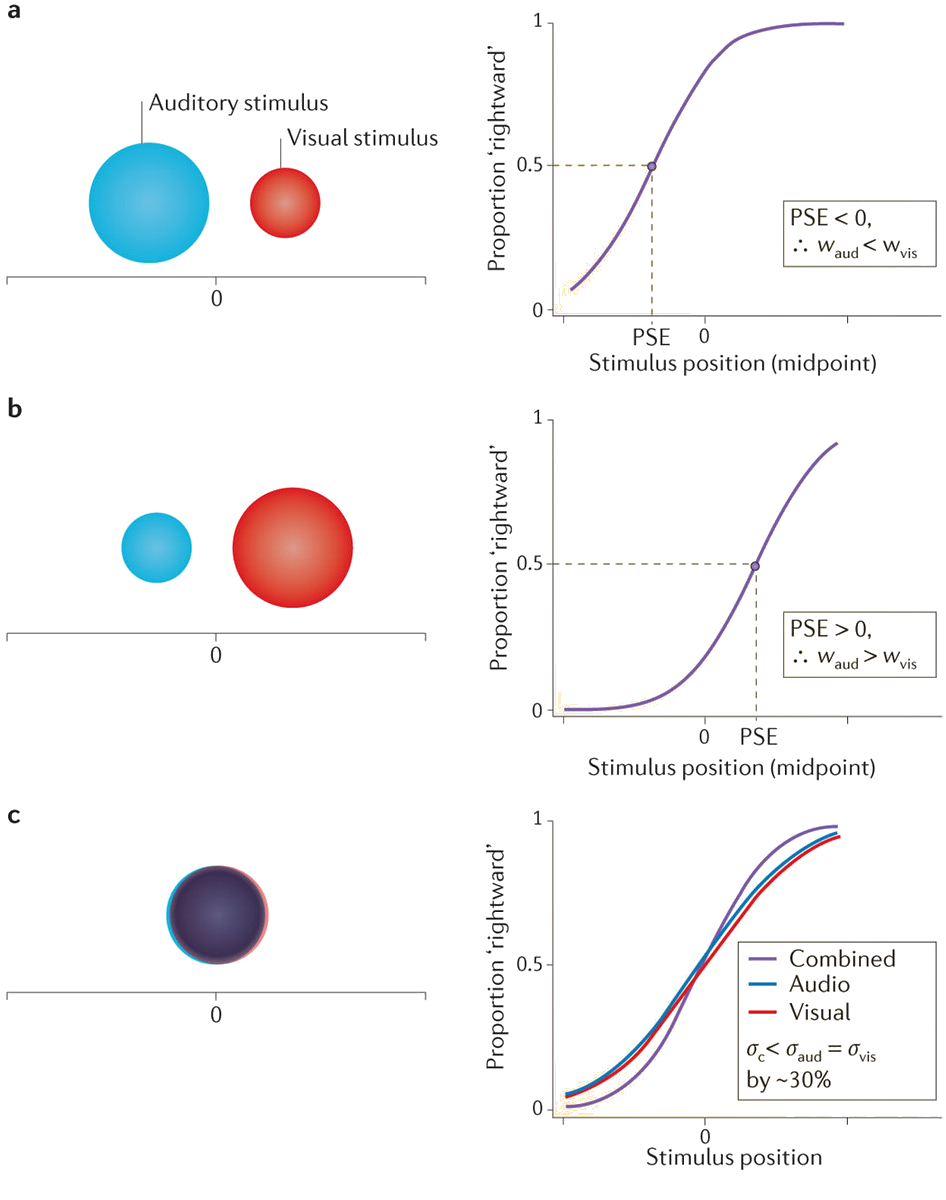
\includegraphics[width=.9\textwidth]{fetsch-visaudloc}
  \caption{Behavioural experiments of visual and auditory localization task. (from \cite{fetsch_bridging_2013})}
  \label{fig:visaudloc}
\end{figure}

In the first experiment (Figure \ref{fig:visaudloc}a), the two modal of stimuli were in conflict position, where the visual stimulus was displaced on the left. Also the visual stimulus was more reliable (depicted by smaller circle) than the auditory stimulus. With the midpoint of the stimuli changed from left to right, the proportion of subjects choosing right increased from 0 to 1. As shown in the figure, the point of subjective equality (PSE), where subjects have equal tendency of left and right, is smaller than 0. This indicates that the visual cue, which is more reliable, dominates more than the auditory cue.

While, in the second experiment (Figure \ref{fig:visaudloc}b), after changing the reliability of the visual stimulus to less than that of the auditory stimulus, the PSE shifted to larger than 0. This also indicates that the more reliable cue dominates more, which is in accord with Equation \ref{eq:optweight} in optimal cue integration.

In the third experiment (Figure \ref{fig:visaudloc}c), the performance of multisensory cue integration was compared against unisenory cue. The visual and auditory stimuli were placed in congruent position with same reliability. Figure shows that the curve of combined cue has steeper slope than that of unisensory cue. In addition, data shows that the standard deviation of combined cue decreased by $30\%$. This is approximate to $1-\sqrt{2}$, which we can calculate using optimal cue integration (Equation \ref{eq:optweight} and \ref{eq:optrel}).

\section{Neurophysiology of multisensory integration}
In parallel to psychophysical studies, neuroscientists try to explain multisensory integration phenomena on account of the neural basis in brains.
They conduct experiments to examine the physiological properties of a neuron or a population of neurons that underlies the integration functions.

Researchers found that multisensory neurons are particularly abundant in the superior colliculus (SC), a midbrain structure primarily involved in orienting the eyes and head towards salient stimuli\cite{sparks_translation_1986}. Another area in brain that caught interest from researchers is the dorsal medial superior temporal area (MSTd), which is responsible for integration visual and vestibular cues for detecting self-motion\cite{gu_visual_2006}.

\subsection{Empirical principles}
By studying the cat SC area for multisensory integration, researchers found a number of empirical principles, which state the properties of multisensory integration\cite{meredith_interactions_1983}. The most prominent principles are the ``inverse effectiveness'' and ``spatial and temporal principle''.

\TODO{details about ``inverse effectiveness'' and ``spatial and temporal principle''.}

\subsection{Development of multisensory integration}
Besides understanding the usage of multisensory integration, plentiful of researches are into knowing how multisensory integration is acquired. 

\TODO{a short overview of physiological study of development of MSI.}

\section{Neural network models}
With the insight from psychophysical and physiological study, a number of computational models, including neural network models are developed. 

\subsection{The normalization model}
Among all computational models of multisensory integration, the normalization model\cite{ohshiro_normalization_2011} is of particular interest. This model helps to explain several key empirical findings: the reliability-dependent combination rule in area MSTd as well as
the empirical principles that were initially described in classic studies of the SC.

\TODO{details of normalization model.}

\subsection{}
\TODO{other models.}

\section{Discussion}
\TODO{summarize current achievement; discuss how these studies can give insight to develop more practical models (artificial systems ?)}

\addcontentsline{toc}{section}{References}
\bibliography{bib}
\bibliographystyle{plain}

\end{document}
